\documentclass[12pt, fleqn]{article}  
\usepackage[T2A]{fontenc}
\usepackage[english,russian]{babel}
\usepackage[utf8]{inputenc}


\usepackage{amsfonts}
\usepackage{amsmath}

\usepackage{graphicx}
\graphicspath{ {jpg/} }
\DeclareGraphicsExtensions{.pdf,.png,.jpg}
\usepackage{float}
\usepackage{subcaption}

\usepackage{xcolor} 
\usepackage{color}

\usepackage{listings} 

\usepackage{caption}
\DeclareCaptionFont{white}{\color{white}} 
\DeclareCaptionFormat{listing}{\colorbox{gray}{\parbox{\textwidth}{#1#2#3}}}
\captionsetup[lstlisting]{format=listing,labelfont=white,textfont=white}

\makeatletter
\renewcommand{\@oddfoot}{\hfill\thepage}
\makeatother

\begin{document}
\begin{titlepage}

\begin{center}
\large ФЕДЕРАЛЬНОЕ ГОСУДАРСТВЕННОЕ БЮДЖЕТНОЕ \linebreak
ОБРАЗОВАТЕЛЬНОЕ УЧРЕЖДЕНИЕ \\ ВЫСШЕГО ОБРАЗОВАНИЯ \\
"МОСКОВСКИЙ ГОСУДАРСТВЕННЫЙ УНИВЕРСИТЕТ \\ имени М.В.ЛОМОНОСОВА"
\end{center}

\begin{center}
\vspace{5mm}\Large МЕХАНИКО-МАТЕМАТИЧЕСКИЙ ФАКУЛЬТЕТ
\end{center}

\begin{center}
\vspace{5mm}\Large 2 КУРС
\end{center}


\begin{center}
\vspace{5mm}\bf\Large{Отчет по задаче №5. Фрактальное сжатие изображений }\linebreak
\vfill
\it{Работу выполнил:\hfil Репин Михаил Денисович студент 224 группы\\}
\it{Семинарист: \hfill Почеревин Роман Владимирович\\}
\today
\end{center}
\end{titlepage}

\setcounter{page}{2}

\tableofcontents{}

\newpage
\section{Условие задачи}

\large {\it Условие:} Реализовать алгоритмы фрактального сжатия и восстановления изображения. Работать с черно-белыми изображениями.
\section{Используемые библиотеки}
Используются библиотеки: \large{\it imageio.v2} для открытия и записи изображений; \large{\it numpy} для удобной работы с числовыми массивами и выполнения математических операций;
библиотека \large{\it  matplotlib} для вывода в одном окне всех итераций распаковки изображения.

  
\section{Алгоритм решения  задачи и элементы кода}Первоначально считываем исходное изображение с помощью функции \large{\it imread} из библиотеки imageio.v2. Затем с помощью функций библиотеки \large{\it numpy} делаем изображенние черно-белым. Вызываем функцию \large{\it compress}, куда в качестве параметров передаем необходимые размеры областей разбиения (о них подробнее ниже), для удобства и быстроты операция берем их за степени двойки. Вводим разбиение матрицы изображения на постоянную сетку (так называемых ранговых квадратов), вводим разбиение на сетку перекрывающихся квадратов (так называемых доменных квадратов). С помщью функции \large{\it alltransform}  генерируем всевозможные афинные преобразования для каждого из доменных блоков, предварительно сжимая их до размеров ранговых блоков. Затем, проходясь по разбиению постоянной сеткой, для каждого из ранговых квадратов подбираем наиболее похожий преобразованный доменный квадрат с точки зрения метрики Фробениуса. Запоминаем координаты и коэффициенты преобразования, записываем их в массив сжатия. На этом процесс сжатия завершен.
\lstset{ %
language=Python,                 % выбор языка для подсветки (python)
basicstyle=\ttfamily\footnotesize, % размер и начертание шрифта для подсветки кода
%basicstyle=\ttm,
keywordstyle=\bfseries\color{green!40!black}, %keywordstyle=\bfseries\color{green!40!black},
identifierstyle=\color{blue},
%basicstyle=\small\sffamily, % размер и начертание шрифта для подсветки кода
numbers=none,               % где поставить нумерацию строк (слева\справа)(none)
%numberstyle=\tiny,           % размер шрифта для номеров строк
%stepnumber=1,                   % размер шага между двумя номерами строк
%numbersep=5pt,                % как далеко отстоят номера строк от подсвечиваемого кода
backgroundcolor=\color{white}, % цвет фона подсветки - используем \usepackage{color}
showspaces=false,            % показывать или нет пробелы специальными отступами
showstringspaces=false,      % показывать или нет пробелы в строках
showtabs=false,             % показывать или нет табуляцию в строках
frame=single,              % рисовать рамку вокруг кода
tabsize=2,                 % размер табуляции по умолчанию равен 2 пробелам
captionpos=t,              % позиция заголовка вверху [t] или внизу [b] 
breaklines=true,           % автоматически переносить строки (да\нет)
breakatwhitespace=false, % переносить строки только если есть пробел
escapeinside={\%*}{*)}   % если нужно добавить комментарии в коде
} 

\begin{lstlisting}[label=Код,caption= Код функции compress]
def compress(img, dsize, rsize, step):
    com_array = []
    transformed_blocks = all_transform(img,dsize, rsize, step)
    i_count = img.shape[0] // rsize
    j_count = img.shape[1] // rsize
    f = open('res.bin', 'wb')
    f.write((str(i_count) + '\n').encode())
    f.write((str(j_count) + '\n').encode())
    for i in range(i_count):
        com_array.append([])
        for j in range(j_count):
            print("{}/{} ; {}/{}".format(i, i_count, j, j_count))
            com_array[i].append(None)
            min_d = float('inf')
            R = img[i*rsize:(i+1)*rsize,j*rsize:(j+1)*rsize]
            for k, l, val, angle, D in transformed_blocks:
                contrast, brightness = bright(R, D)
                D = contrast*D + brightness
                d = np.sum(np.square(R - D))
                if d < min_d:
                    min_d = d
                    com_array[i][j] = (k, l, val, angle, contrast, brightness)
            for t in range(len(com_array[i][j])):
                if t != len(com_array[i][j])-1:
                    f.write((str(com_array[i][j][t])).encode())
                else:
                    f.write((str(com_array[i][j][t])+'\n').encode())
    f.close()
    return com_array
\end{lstlisting}
\newpage
Функция генерации всевозможных афинных преобразований для доменных квадратов:
\begin{lstlisting}[label=Код,caption= Функция alltransform]
def all_transform(img, dsize, rsize, step):
    factor = dsize // rsize
    transformed_blocks = []
    for i in range((img.shape[0] - dsize) // step + 1):
        for j in range((img.shape[1] - dsize) // step + 1):
            cp_block = reduce(img[i*step:i*step+dsize, j*step:j*step+dsize], factor)
            for val, angle in candidates:
                transformed_blocks.append((i, j, val, angle, make_transform(cp_block, val, angle)))
    return transformed_blocks
\end{lstlisting}


Алгоритм распаковки генерирует совершенно случайную картинку (в данном случае полностью черную). Затем, разбивая картинку на ранговые и доменные блоки, применяет соответствующее преобразование из сжатых данных для соответствующего доменного блока и вставляет получившийся кусок на место рангового блока. Такая система итерируемых функций применяется к картинке заданное число раз(как видно, 10 раз уже достаточно). В итоге получется исходная картинка, с допустимыми для данного алгоритма потерями.
\newpage
\begin{lstlisting}[label=Код,caption= Распаковка изображения]
def decompress(com_array, dsize, rsize, step, nb_iter=10):
    factor = dsize // rsize
    height = len(com_array) * rsize
    width = len(com_array[0]) * rsize
    iterations = [np.full((height, width), 1)]
    cur_img = np.zeros((height, width))
    for i_iter in range(nb_iter):
        print(i_iter)
        for i in range(len(com_array)):
            for j in range(len(com_array[i])):
                k, l, flip, angle, contrast, brightness = com_array[i][j]
                D = reduce(iterations[-1][k*step:k*step+dsize, l*step:l*step+dsize], factor)
                R = make_transform(D, flip, angle, contrast, brightness)
                cur_img[i*rsize:(i+1)*rsize, j*rsize:(j+1)*rsize] = R
        iterations.append(cur_img)
        cur_img = np.zeros((height, width))
    return iterations
\end{lstlisting}

\begin{figure}[H]
\section{Примеры работы алгоритма}
\begin{center}
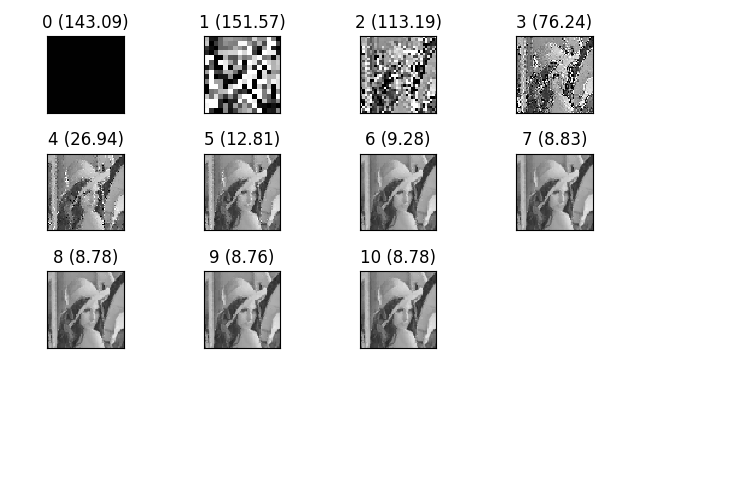
\includegraphics[width=460pt,height=350pt]{example.png}
\caption{Итерации распаковки изображения}
\end{center}
\end{figure}

\end{document}